%

\documentclass{article}

\usepackage{geometry}
\usepackage{layout}
\geometry{
  left=2.0cm,
  right=2.5cm,
  top=3.5cm,
  bottom=3cm
}
\usepackage{graphics}
\usepackage{longtable}
\usepackage{fancyhdr}
\usepackage{url}

\newcommand{\eqdef}{\stackrel{def}{=}}

%\setlength\parindent{0pt}

%

\newcommand{\xapi}{\textsc{XAPI}}
\newcommand{\xen}{\textsc{Xen}}
%% Document title
\newcommand{\doctitle}{Evolving the XenAPI}

%% Document date
\newcommand{\datestring}{7th May 2010}

\newcommand{\releasestatement}{Comments are welcome!}

%% Document revision
\newcommand{\revstring}{Document Revision 0.1}

%% Document authors
\newcommand{\docauthors}{
%David Scott: & {\tt dave.scott@eu.citrix.com}
}
\newcommand{\legalnotice}{Copyright \copyright{} 2010 Citrix, Inc.\\ \\
Permission is granted to copy, distribute and/or modify this document under
the terms of the GNU Free Documentation License, Version 1.2 or any later
version published by the Free Software Foundation; with no Invariant Sections,
no Front-Cover Texts and no Back-Cover Texts.  A copy of the license is
included in the section entitled "GNU Free Documentation License".
}



\begin{document}

% The coversheet itself
%
% Copyright (c) 2006-2007 XenSource, Inc.
%
% All rights reserved.
%
% Authors: Ewan Mellor, Richard Sharp, Dave Scott, Jon Harrop.
%

\pagestyle{empty}

\doctitle{} \hfill \revstring{}

\vspace{1cm}

\begin{center}
\resizebox{8cm}{!}{\includegraphics{\coversheetlogo}}

\vspace{2cm}

\begin{Huge}
  \doctitle{}
\end{Huge}

\vspace{1cm}
\begin{Large}
\revstring{}\\
\releasestatement{}

\vspace{1cm}
\begin{tabular}{rl}
\docauthors{}
\end{tabular}
\end{Large}
\end{center}
\vspace{.5cm}

\vfill

\noindent
\legalnotice{}

\newpage
\pagestyle{fancy}

% ... and off we go!

\section{Introduction}

We wish to:
\begin{enumerate}
\item allow VM memory to be adjusted dynamically without having to reboot; and
\item ``squeeze'' a few more VMs onto a host to cover the interval between another host failing and more capacity being brought online.
\end{enumerate}

\squeezed{} is a per-host memory ballooning daemon. It performs two tasks:
\begin{enumerate}
\item it exports a simple host memory management interface to the \xapi{} toolstack through which \xapi{} can {\em reserve} memory for new domains;
\item it applies a {\em ballooning policy} to all domains running on a host.
\end{enumerate}
The daemon currently includes a simple ballooning policy (see Section~\ref{Ballooning policy}) and the intention is that this can be replaced later with more sophisticated policies (e.g.\ {\em xenballoond}\footnote{\url{http://wiki.xensource.com/xenwiki/Open_Topics_For_Discussion?action=AttachFile&do=get&target=Memory+Overcommit.pdf}})). Although the only client is the \xapi{} toolstack, the interface can in theory be used by other clients.

In the short-term this document will allow the assumptions and the design to be reviewed. In the longer term this document will become part of the \xapi{} toolstack software design notes.

The rest of this document is structured as follows. Section~\ref{assumptions} lists assumptions made by the ballooning daemon on other parts of the system; these assumptions need careful review and may not be valid. Section~\ref{Toolstack interface} describes the interface between the toolstack and the ballooning daemon. Section~\ref{Ballooning policy} describes the simple built-in ballooning policy and Section~\ref{memory model} describes how \squeezed{} models memory. The main loop of the daemon is described in Section~\ref{The main loop} and a detailed example is described in Section~\ref{example}. Section~\ref{structure} describes the structure of the daemon itself and finally Section~\ref{issues} lists some known issues.

\section{Environmental assumptions}
\label{assumptions}
\begin{enumerate}
\item The \squeezed{} daemon runs within a \xen{} domain 0 and communicates to xenstored via a Unix domain socket. Therefore \squeezed{} is granted full access to xenstore, enabling it to modify every domain's \texttt{memory/target}.

\item The \squeezed{} daemon calls \texttt{setmaxmem} in order to cap the amount of memory a domain can use. This relies on a patch to xen\footnote{\url{http://xenbits.xen.org/xapi/xen-3.4.pq.hg?file/c01d38e7092a/max-pages-below-tot-pages}} which allows \texttt{maxmem}
 to be set lower than \texttt{totpages}. See Section~\ref{maxmem} for more information.

\item The \squeezed{} daemon assumes that only domains which write \texttt{control/feature-balloon} into xenstore can respond to ballooning requests. It will not ask any other domains to balloon.

\item The \squeezed{} daemon assumes that the memory used by a domain is: (i) that listed in \texttt{domain\_getinfo} as \texttt{totpages}; (ii) shadow as given by \texttt{shadow\_allocation\_get}; and (iii) a small (few KiB) of miscellaneous \xen{} structures (e.g.\ for domains, vcpus) which are invisible.

\item The \squeezed{} daemon assumes that a domain which is created with a particular \texttt{memory/target} (and \texttt{startmem}, to within rounding error) will reach a stable value of \texttt{totpages} before writing \texttt{control/feature-balloon}.\footnote{%
The \texttt{control/feature-balloon} key is probably the wrong signal.
}%
The daemon writes this value to \texttt{memory/memory-offset} for future reference.
\begin{itemize}
\item The \squeezed{} daemon does not know or care exactly what causes the difference between \texttt{totpages} and \texttt{memory/target} and it does {\em not} expect it to remain constant across \xen{} releases. It only expects the value to remain constant over the lifetime of a domain.
\end{itemize}

\item The \squeezed{} daemon assumes that the balloon driver has hit its target when difference between \texttt{memory/target} and \texttt{totpages} equals the \texttt{memory-offset} value.
\begin{itemize}
\item Corrollary: to make a domain with a responsive balloon driver currenty using \texttt{totpages} allocate or free $x$, it suffices to set \texttt{memory/target} to $x+\texttt{totpages}+\texttt{memory-offset}$ and wait for the balloon driver to finish. See Section~\ref{memory model} for more detail.
\end{itemize}
\item The \squeezed{} daemon must maintain a ``slush fund'' of memory (currently 9MiB) which it must prevent any domain from allocating. Since (i) some \xen{} operations (such as domain creation) require memory within a physical address range (e.g. $<$ 4GiB) and (ii) since \xen{} preferentially allocates memory outside these ranges, it follows that by preventing guests from allocating {\em all} host memory (even transiently) we guarantee that memory from within these special ranges is always available. See Section~\ref{twophase section} for more details.

\item The \squeezed{} daemon assumes that it may set \texttt{memory/target} to any value within range: \texttt{memory/dynamic-max} to \texttt{memory/dynamic-min}

\item The \squeezed{} daemon assumes that the probability of a domain booting successfully may be increased by setting \texttt{memory/target} closer to \texttt{memory/static-max}.

\item The \squeezed{} daemon assumes that, if a balloon driver has not made any visible progress after 5 seconds, it is effectively {\em inactive}. Active domains will be expected to pick up the slack.
\end{enumerate}

\section{Toolstack interface}
\label{Toolstack interface}

This section begins by describing the concept of a {\em reservation} and then describes the toolstack interface in pseudocode.

A {\em reservation} is: an amount of host free memory tagged with an associated {\em reservation id}.
Note this is an internal \squeezed{} concept and \xen{} is completely unaware of it. When the daemon is moving memory between domains, it always aims to keep 
\[
\mathit{host\ free\ memory} >= s + \sum_i{\mathit{reservation}_i}
\]
where $s$ is the size of the ``slush fund'' (currently 9MiB) and $\mathit{reservation}_i$ is the amount corresponding to the $i$th reservation.

As an aside:
Earlier versions of \squeezed{} always associated memory with a \xen{} domain. Unfortunately this required domains to be created before memory was freed which was problematic because domain creation requires small amounts of contiguous frames. Rather than implement some form of memory defragmentation, \squeezed{} and \xapi{} were modified to free memory before creating a domain. This necessitated making memory {\em reservations} first-class stand-alone entities.


Once a {\em reservation} is made (and the corresponding memory is freed), it can be {\em transferred} to a domain created by a toolstack. This associates the {\em reservation} with that domain so that, if the domain is destroyed, the {\em reservation} is also freed. Note that \squeezed{} is careful not to count both a domain's {\em reservation} and its \texttt{totpages} during e.g. domain building: instead it considers the domain's allocation to be the maximum of {\em reservation} and \texttt{totpages}.

The size of a {\em reservation} may either be specified exactly by the caller or the caller may provide a memory range. If a range is provided the daemon will allocate at least as much as the minimum value provided and as much as possible up to the maximum. By allocating as much memory as possible to the domain, the probability of a successful boot is increased.

Clients of the \squeezed{} provide a string name when they log in. All untransferred reservations made by a client are automatically deleted when a client logs in. This prevents memory leaks where a client crashes and loses track of its own reservation ids.

The interface looks like this:
\begin{verbatim}
string session_id login(string client_name)

string reservation_id reserve_memory(string client_name, int kib)
int amount, string reservation_id reserve_memory_range(string client_name, int min, int max)

void delete_reservation(string client_name, string reservation_id)

void transfer_reservation_to_domain(string client_name, string reservation_id, int domid)
\end{verbatim}

The \xapi{} toolstack has code like the following: (in \url{http://www.xen.org/files/XenCloud/ocamldoc/index.html?c=xapi&m=Vmops})
\begin{verbatim}
 r_id = reserve_memory_range("xapi", min, max);
 try:
    d = domain_create()
    transfer_reservation_to_domain("xapi", r_id, d)
 with:
    delete_reservation("xapi", r_id)
\end{verbatim}

The interface is currently implemented using a trivial RPC protocol over xenstore where requests and responses are directories and their parameters and return values are keys in those directories.

\section{Ballooning policy}
\label{Ballooning policy}
This section describes the very simple default policy currently built-into \squeezed{}.

Every domain has a pair of values written into xenstore: \texttt{memory/dynamic-min} and \texttt{memory/dynamic-max} with the following meanings:
\begin{description}
\item[\texttt{memory/dynamic-min}]: the lowest value that \squeezed{} is allowed to set \texttt{memory/target}. The administrator should make this as low as possible but high enough to ensure that the applications inside the domain actually work.
\item[\texttt{memory/dynamic-max}]: the highest value that \squeezed{} is allowed to set \texttt{memory/target}. This can be used to dynamically cap the amount of memory a domain can use.
\end{description}
If all balloon drivers are responsive then \squeezed{} daemon allocates memory proportionally, so that each domain has the same value of:
\[
\frac{
\texttt{memory/target}-\texttt{memory/dynamic-min}
}{
\texttt{memory/dynamic-max}-\texttt{memory/dynamic-min}
}
\]
So:
\begin{itemize}
\item if memory is plentiful then all domains will have $\texttt{memory/target}=\texttt{memory/dynamic-max}$
\item if memory is scarce then all domains will have $\texttt{memory/target}=\texttt{memory/dynamic-min}$
\end{itemize}
Note that the values of \texttt{memory/target} suggested by the policy are ideal values. In many real-life situations (e.g. when a balloon driver fails to make progress and is declared {\em inactive}) the \texttt{memory/target} values will be different.

Note that, by default, domain 0 has $\texttt{dynamic\_min}=\texttt{dynamic\_max}$, effectively disabling ballooning.  Clearly a more sophisticated policy would be required here since ballooning down domain 0 as extra domains are started would be\ldots{} problematic.

\section{The memory model used by \squeezed{}}
\label{memory model}
This section describes the model used internally by \squeezed{}.

The \squeezed{} daemon considers a ballooning-aware domain (i.e.\ one which has written the \texttt{feature-balloon} flag into xenstore) to be a 6-tuple:
\[
\mathit{ballooning~domain} = (\texttt{dynamic-min}, \texttt{dynamic-max}, \texttt{target}, \texttt{totpages}, \texttt{memory-offset}, \texttt{maxmem})
\]
where
\begin{description}
\item[\texttt{dynamic-min}]: policy value written to \texttt{memory/dynamic-min} in xenstore by a toolstack (see Section~\ref{Ballooning policy})
\item[\texttt{dynamic-max}]: policy value written to \texttt{memory/dynamic-max} in xenstore by a toolstack (see Section~\ref{Ballooning policy})
\item[\texttt{target}]: balloon driver target written to \texttt{memory/target} in xenstore by \squeezed{}
\item[\texttt{totpages}]: instantaneous number of pages used by the domain as returned by \texttt{domain\_getinfo}
\item[\texttt{memory-offset}]: constant difference between \texttt{target} and \texttt{totpages} when the balloon driver believes no ballooning is necessary:
\[
\texttt{memory-offset} \eqdef \texttt{totpages} - \texttt{target} \mathit{~when~idle}
\]
\item[\texttt{maxmem}]: upper limit on \texttt{totpages}:
\[
\texttt{totpages} <= \texttt{maxmem}
\]
\end{description}
For convenience we define a \texttt{totpages'} to be the target value necessary to cause a domain currently using \texttt{totpages} to maintain this value indefinitely.
\[
\texttt{totpages'} \eqdef \texttt{totpages} - \texttt{memory-offset}
\]

The \squeezed{} daemon believes that:
\begin{itemize}
\item a domain should be ballooning iff $\texttt{totpages'} <> \texttt{target}$ (unless it has become {\em inactive});
\item a domain has hit its target iff $\texttt{totpages'} = \texttt{target}$ (to within 1 page);
\item if a domain has $\texttt{target}\leftarrow x$ then, when ballooning is complete, it will have $\texttt{totpages}=\texttt{memory-offset}+x$; and therefore
\item to cause a domain to free $y$ it sufficies to set $\texttt{target}\leftarrow\texttt{totpages}-\texttt{memory-offset}-y$.
\end{itemize}

The \squeezed{} daemon considers non-ballooning aware domains (i.e.\ those which have not written \texttt{feature-balloon}) to be represented by pairs of:
\[
\mathit{other~domain} = (\texttt{totpages}, \mathit{reservation})
\]
where
\begin{description}
\item[\texttt{totpages}]: instantaneous number of pages used by the domain
  as returned by \texttt{domain\_getinfo}
\item[$\mathit{reservation}$]: memory initially freed for this domain by
  \squeezed{} after a \texttt{transfer\_reservation\_to\_domid} call
\end{description}
Note that non-ballooning aware domains will always have
$\texttt{startmem}=\texttt{target}$ since the domain will not be instructed
to balloon. Since a domain which is being built will have
$0<=\texttt{totpages}<=\mathit{reservation}$, \squeezed{} computes:
\[
\mathit{unused}(i) \eqdef i.\mathit{reservation} - i.\texttt{totpages}
\]
and subtracts this from its model of the host's free memory, ensuring that it doesn't accidentally reallocate this memory for some other purpose.


The \squeezed{} daemon believes that:
\begin{itemize}
\item all guest domains start out as non-ballooning aware domains where $\texttt{target}=\mathit{reservation}=\texttt{startmem}$;
\item some guest domains become ballooning-aware during their boot sequence i.e.\ when they write \texttt{feature-balloon}
\end{itemize}

The \squeezed{} daemon considers a host to be a 5-tuple:
\[
\mathit{host} = (\mathit{ballooning~domains}, \mathit{other~domains}, s, \texttt{physinfo.free\_pages}, \mathit{reservation}_i)
\]
where
\begin{description}
\item[$\mathit{ballooning~domains}$]: a list of $\mathit{ballooning~domain}$
  values representing domains which \squeezed{} will instruct to balloon;
\item[$\mathit{other~domains}$]: a list of $\mathit{other~domain}$ values
  which includes both domains which are still booting and will transform
  into $\mathit{ballooning~domains}$ and those which have no balloon drivers.
\item[$s$]: a ``slush fund'' of low memory required for \xen{};
\item[\texttt{physinfo.free\_pages}]: total amount of memory instantanously free (including both \texttt{free\_pages} and \texttt{scrub\_pages})
\item[$\mathit{reservation}_i$]: a set of memory {\em reservations} not allocated to any domain
\end{description}
The \squeezed{} daemon considers memory to be unused (i.e.\ not allocated for any useful purpose) as follows:
\[
\mathit{unused~memory} = \texttt{physinfo.free\_pages} -
\Sigma_i\mathit{reservation}_i - s - \Sigma_{i\in\mathit{other~domains}}\mathit{unused}(i)
\]

\section{The main loop}
\label{The main loop}

The main loop \footnote{\texttt{change\_host\_free\_memory} in \url{http://xenbits.xen.org/xapi/xen-api.hg?file/3e8c0167940d/ocaml/xenops/squeeze.ml}}  is triggered by either:
\begin{enumerate}
\item the arrival of an allocation request on the toolstack interface; or
\item the policy engine -- polled every 10s -- deciding that a target adjustment is needed.
\end{enumerate}
Each iteration of the main loop\footnote{\texttt{one\_iteration} in \url{http://xenbits.xen.org/xapi/xen-api.hg?file/3e8c0167940d/ocaml/xenops/squeeze.ml}} generates the following actions:
\begin{enumerate}
\item Domains which were active but have failed to make progress towards their target in 5s are declared {\em inactive}. These domains then have:
\[
\texttt{maxmem}\leftarrow\mathit{min}(\texttt{target}, \texttt{totpages})
\]
\item Domains which were inactive but have started to make progress towards their target are declared {\em active}. These domains then have:
\[
\texttt{maxmem}\leftarrow\texttt{target}
\]
\item Domains which are currently active have new targets computed according to the policy (see Section~\ref{Ballooning policy}). Note that inactive domains are ignored and not expected to balloon.
\end{enumerate}
Note that domains remain classified as {\em inactive} only during one run of the main loop. Once the loop has terminated all domains are optimistically assumed to be {\em active} again. Therefore should a domain be classified as {\em inactive} once, it will get many later chances to respond.

See Section~\ref{twophase section} for more detail on how targets are updated and Section~\ref{maxmem} for more detail about \texttt{maxmem}.

The main loop has a notion of a host free memory ``target'', similar to the existing domain memory \texttt{target}. When we are trying to free memory (e.g. for starting a new VM), the host free memory ``target'' is increased. When we are trying to distribute memory among guests (e.g.\ after a domain has shutdown and freed lots of memory), the host free memory ``target'' is low. Note the host free memory ``target'' is always at least several MiB to ensure that some host free memory  with physical address $<$ 4GiB is free (see Section~\ref{twophase section} for related information).

The main loop terminates when all {\em active} domains have reached their targets (this could be because all domains responded or because they all wedged and became inactive); and the policy function hasn't suggested any new target changes. There are three possible results:
\begin{enumerate}
\item Success if the host free memory is near enough its ``target'';
\item Failure if the operation is simply impossible within the policy limits (i.e. \texttt{dynamic\_min} values are too high;
\item Failure if the operation failed because one or more domains became {\em inactive} and this prevented us from reaching our host free memory ``target''.
\end{enumerate}
Note that, since only {\em active} domains have their targets set, the system effectively rewards domains which refuse to free memory ({\em inactive}) and punishes those which do free memory ({\em active}). This effect is countered by signalling to the admin which domains/VMs aren't responding so they can take corrective action.
To achieve this, the daemon monitors the list of {\em inactive} domains and if a domain is {\em inactive} for more than 20s it writes a flag into xenstore \texttt{memory/uncooperative}. This key is seen by the \xapi{} toolstack which currently generates an alert to inform the admin.


\subsection{Two-phase target setting}
\label{twophase section}

\begin{figure}
\begin{center}
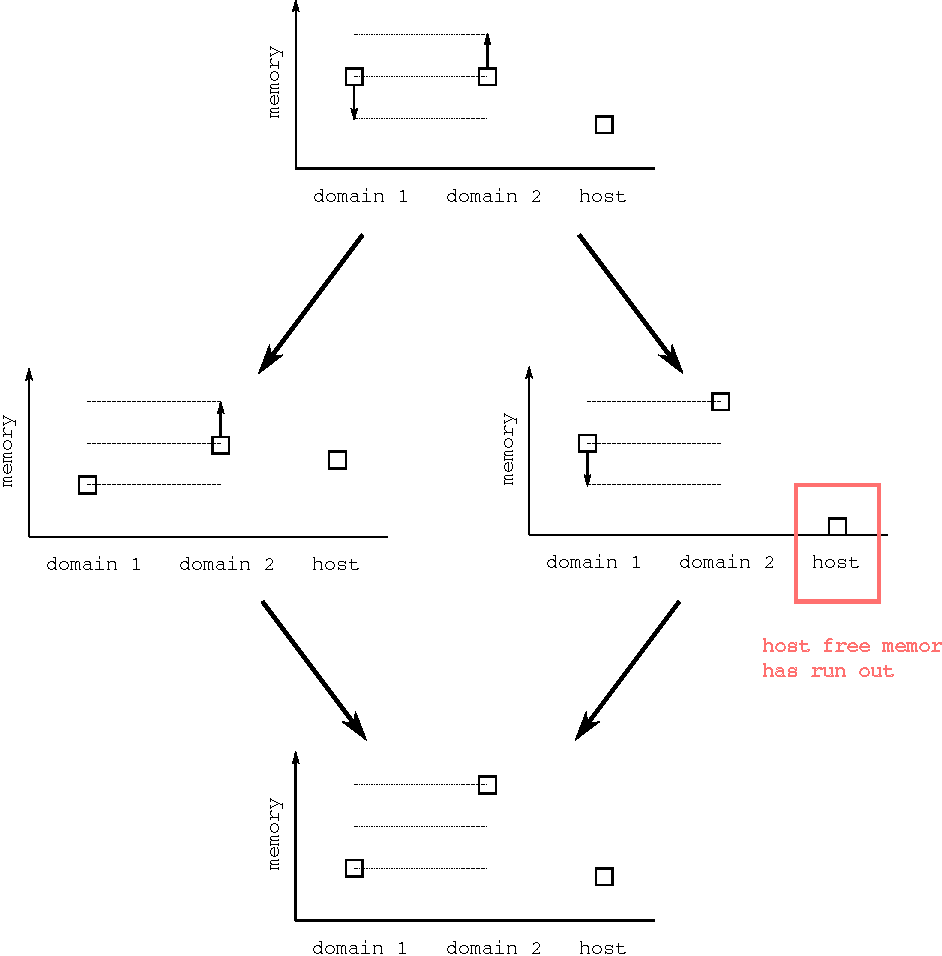
\includegraphics{fig/twophase}
\end{center}
\caption{The diagram shows how a system with two domains can evolve if domain \texttt{memory/target} values are increased for some domains and decreased for others, at the same time. Each graph shows two domains (domain 1 and domain 2) and a host. For a domain, the square box shows its $\texttt{totpages'}$ and the arrow indicates the direction of the \texttt{memory/target}. For the host the square box indicates total free memory. Note the highlighted state where the host's free memory is temporarily exhausted.}
\label{twophase}
\end{figure}

Consider the scenario shown graphically in Figure~\ref{twophase}. In the initial state (at the top of the diagram), there are two domains, one which has been requested to use more memory and the other requested to use less memory. In effect the memory is to be transferred from one domain to the other. In the final state (at the bottom of the diagram), both domains have reached their respective targets, the memory has been transferred and the host free memory is at the same value it was initially. However the system will not move atomically from the initial state to the final: there are a number of possible transient in-between states, two of which have been drawn in the middle of the diagram. In the left-most transient state the domain which was asked to {\em free} memory has freed all the memory requested: this is reflected in the large amount of host memory free. In the right-most transient state the domain which was asked to {\em allocate} memory has allocated all the memory requested: now the host's free memory has hit zero. 

If the host's free memory hits zero then \xen{} has been forced to give all memory to guests, including memory $<$ 4GiB which is critical for allocating certain structures. Even if we ask a domain to free memory via the balloon driver there is no guarantee that it will free the {\em useful} memory. This leads to an annoying failure mode where operations such as creating a domain free due to \texttt{ENOMEM} despite the fact that there is apparently lots of memory free.

The solution to this problem is to adopt a two-phase \texttt{memory/target} setting policy. The \squeezed{} daemon forces domains to free memory first before allowing domains to allocate, in-effect forcing the system to move through the left-most state in the diagram above.


\subsection{Use of \texttt{maxmem}}
\label{maxmem}

The \xen{} domain \texttt{maxmem} value is used to limit memory allocations by the domain. The rules are:
\begin{enumerate}
\item if the domain has never been run and is paused then $\texttt{maxmem}\leftarrow\texttt{reservation}$ (for information about reservations see Section~\ref{Toolstack interface});
\begin{itemize}
\item these domains are probably still being built and we must let them allocate their \texttt{startmem}
\item \textbf{FIXME}: this ``never been run' concept pre-dates the \texttt{feature-balloon} flag: perhaps we should use the \texttt{feature-balloon} flag instead.
\end{itemize}
\item if the domain is running and the balloon driver is thought to be working then $\texttt{maxmem}\leftarrow\texttt{target}$; and
\begin{itemize}
\item there may be a delay between lowering a target and the domain noticing so we prevent the domain from allocating memory when it should in fact be deallocating.
\end{itemize}
\item if the domain is running and the balloon driver is thought to be inactive then $\texttt{maxmem}\leftarrow \mathit{min}(\texttt{target}, \texttt{actual})$.
\begin{itemize}
\item if the domain is using more memory than it should then we allow it to make progress down towards its target; however
\item if the domain is using less memory than it should then we must prevent it from suddenly waking up and allocating more since we have probably just given it to someone else
\item \textbf{FIXME}: should we reduce the target to leave the domain in a neutral state instead of asking it to allocate and fail forever?
\end{itemize}
\end{enumerate}
   
\section{Example operation}
\label{example}

\begin{figure}
\begin{center}
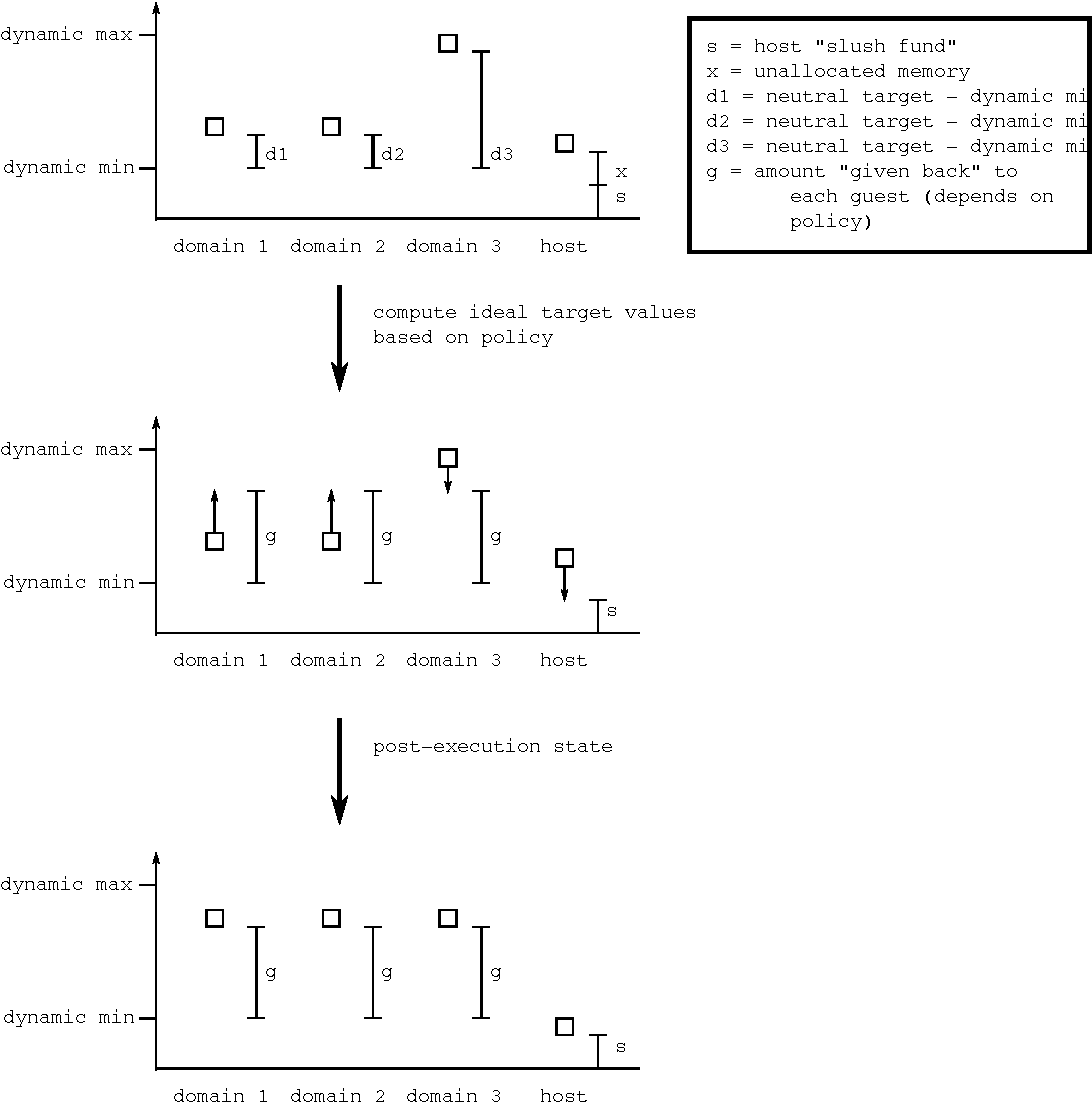
\includegraphics{fig/calculation}
\end{center}
\caption{The diagram shows an initial system state comprising 3 domains on a single host. The state is not ideal; the domains each have the same policy settings (\texttt{dynamic-min} and \texttt{dynamic-max}) and yet are using differing values of $\texttt{totpages'}$. 
 In addition the host has more memory free than desired. The second diagram shows the result of computing ideal target values and the third diagram shows the result after targets have been set and the balloon drivers have responded.}
\label{calculation}
\end{figure}

The scenario in Figure~\ref{calculation} includes 3 domains (domain 1, domain 2, domain 3) on a host. Each of the domains has a non-ideal $\texttt{totpages'}$ value.

 Recall we also have the policy constraint that:
\[
\texttt{dynamic-min} <= \texttt{target} <= \texttt{dynamic-max}
\]
Hypothetically if we reduce \texttt{target} by $\texttt{target}-\texttt{dynamic-min}$ (i.e. by setting $\texttt{target}\leftarrow\texttt{dynamic-min}$) then we should reduce \texttt{totpages} by the same amount, freeing this much memory on the host. In the upper-most graph in Figure~\ref{calculation} the total amount of memory which would be freed if we set each of the 3 domain's $\texttt{target}\leftarrow\texttt{dynamic-min}$ is:
\[
\mathit{d1} + \mathit{d2} + \mathit{d3}
\]
In this hypothetical situation we would now have $x + s + \mathit{d1} + \mathit{d2} + \mathit{d3}$ free on the host where $s$ is the host slush fund and $x$ is completely unallocated. Since we always want to keep the host free memory above $s$, we are free to return $x + \mathit{d1} + \mathit{d2} + \mathit{d3}$ to guests. If we use the default built-in proportional policy then, since all domains have the same \texttt{dynamic-min} and \texttt{dynamic-max}, each gets the same fraction of this free memory which we call $g$:
\[
g \eqdef \frac{x + \mathit{d1} + \mathit{d2} + \mathit{d3}}{3}
\]
For each domain, the ideal balloon target is now $\texttt{target} = \texttt{dynamic-min} + g$. The \squeezed{} daemon sets these targets in two phases, as described in Section~\ref{twophase section}

\section{The structure of the daemon}
\label{structure}
The \squeezed{} daemon is a single-threaded daemon which is started by an \texttt{init.d} script. It sits waiting for incoming requests on its toolstack interface and checks every 10s whether all domain targets are set to the ideal values (see Section~\ref{Ballooning policy}). If an allocation request arrives or if the domain targets require adjusting then it calls into the module \url{ocaml/xenops/squeeze_xen.ml}\footnote{\url{http://www.xen.org/files/XenCloud/ocamldoc/index.html?c=xenops&m=Squeeze_xen}}.

The module \url{ocaml/xenops/squeeze_xen.ml} contains code which inspects the state of the host (through hypercalls and reading xenstore) and creates a set of records describing the current state of the host and all the domains. Note this snapshot of state is not atomic -- it is pieced together from multiple hypercalls and xenstore reads -- we assume that the errors generated are small and we ignore them.
 These records are passed into the \url{ocaml/xenops/squeeze.ml}\footnote{\url{http://www.xen.org/files/XenCloud/ocamldoc/index.html?c=xenops&m=Squeeze}} module where they are processed and converted into a list of {\em actions} i.e. (i) updates to \texttt{memory/target} and; (ii) declarations that particular domains have become {\em inactive} or {\em active}. The rationale for separating the \xen{} interface from the main ballooning logic was to make testing easier: the module \url{ocaml/xenops/squeeze_test.ml}\footnote{\url{http://www.xen.org/files/XenCloud/ocamldoc/index.html?c=xenops&m=Squeeze_test}} contains a simple simulator which allows various edge-cases to be checked.

\section{Issues}
\label{issues}
\begin{itemize}
\item If a linux domU kernel has the netback, blkback or blktap modules then they away pages via \texttt{alloc\_empty\_pages\_and\_pagevec()} during boot. This interacts with the balloon driver to break the assumption that, reducing the target by $x$ from a neutral value should free $x$ amount of memory.
\item Polling the state of the host (particular the xenstore contents) is a bit inefficient. Perhaps we should move the policy values \texttt{dynamic\_min} and \texttt{dynamic\_max} to a separate place in the xenstore tree and use watches instead.
\item The memory values given to the domain builder are in units of MiB. We may wish to similarly quantise the \texttt{target} value or check that the \texttt{memory-offset} calculation still works.
\item The \xen{} patch queue reintroduces the lowmem emergency pool\footnote{\url{http://xenbits.xen.org/xapi/xen-3.4.pq.hg?file/c01d38e7092a/lowmem-emergency-pool}}. This was an attempt to prevent guests from allocating lowmem before we switched to a two-phase target setting procedure. This patch can probably be removed.
\item It seems unnecessarily evil to modify an {\em inactive} domain's \texttt{maxmem} leaving $\texttt{maxmem}<\texttt{target}$, causing the guest to attempt allocations forwever. It's probably neater to move the \texttt{target} at the same time.
\item Declaring a domain {\em active} just because it makes small amounts of progress shouldn't be enough. Otherwise a domain could free 1 byte (or maybe 1 page) every 5s.
\item Likewise, declaring a domain ``uncooperative'' only if it has been {\em inactive} for 20s means that a domain could alternate between {\em inactive} for 19s and {\em active} for 1s and not be declared ``uncooperative''.
\end{itemize}
\appendix{}

\chapter{GNU Free Documentation License}
%\label{label_fdl}

 \begin{center}

       Version 1.2, November 2002


 Copyright \copyright 2000,2001,2002  Free Software Foundation, Inc.
 
 \bigskip
 
     51 Franklin St, Fifth Floor, Boston, MA  02110-1301  USA
  
 \bigskip
 
 Everyone is permitted to copy and distribute verbatim copies
 of this license document, but changing it is not allowed.
\end{center}


\begin{center}
{\bf\large Preamble}
\end{center}

The purpose of this License is to make a manual, textbook, or other
functional and useful document "free" in the sense of freedom: to
assure everyone the effective freedom to copy and redistribute it,
with or without modifying it, either commercially or noncommercially.
Secondarily, this License preserves for the author and publisher a way
to get credit for their work, while not being considered responsible
for modifications made by others.

This License is a kind of "copyleft", which means that derivative
works of the document must themselves be free in the same sense.  It
complements the GNU General Public License, which is a copyleft
license designed for free software.

We have designed this License in order to use it for manuals for free
software, because free software needs free documentation: a free
program should come with manuals providing the same freedoms that the
software does.  But this License is not limited to software manuals;
it can be used for any textual work, regardless of subject matter or
whether it is published as a printed book.  We recommend this License
principally for works whose purpose is instruction or reference.


\begin{center}
{\Large\bf 1. APPLICABILITY AND DEFINITIONS}
\addcontentsline{toc}{section}{1. APPLICABILITY AND DEFINITIONS}
\end{center}

This License applies to any manual or other work, in any medium, that
contains a notice placed by the copyright holder saying it can be
distributed under the terms of this License.  Such a notice grants a
world-wide, royalty-free license, unlimited in duration, to use that
work under the conditions stated herein.  The \textbf{"Document"}, below,
refers to any such manual or work.  Any member of the public is a
licensee, and is addressed as \textbf{"you"}.  You accept the license if you
copy, modify or distribute the work in a way requiring permission
under copyright law.

A \textbf{"Modified Version"} of the Document means any work containing the
Document or a portion of it, either copied verbatim, or with
modifications and/or translated into another language.

A \textbf{"Secondary Section"} is a named appendix or a front-matter section of
the Document that deals exclusively with the relationship of the
publishers or authors of the Document to the Document's overall subject
(or to related matters) and contains nothing that could fall directly
within that overall subject.  (Thus, if the Document is in part a
textbook of mathematics, a Secondary Section may not explain any
mathematics.)  The relationship could be a matter of historical
connection with the subject or with related matters, or of legal,
commercial, philosophical, ethical or political position regarding
them.

The \textbf{"Invariant Sections"} are certain Secondary Sections whose titles
are designated, as being those of Invariant Sections, in the notice
that says that the Document is released under this License.  If a
section does not fit the above definition of Secondary then it is not
allowed to be designated as Invariant.  The Document may contain zero
Invariant Sections.  If the Document does not identify any Invariant
Sections then there are none.

The \textbf{"Cover Texts"} are certain short passages of text that are listed,
as Front-Cover Texts or Back-Cover Texts, in the notice that says that
the Document is released under this License.  A Front-Cover Text may
be at most 5 words, and a Back-Cover Text may be at most 25 words.

A \textbf{"Transparent"} copy of the Document means a machine-readable copy,
represented in a format whose specification is available to the
general public, that is suitable for revising the document
straightforwardly with generic text editors or (for images composed of
pixels) generic paint programs or (for drawings) some widely available
drawing editor, and that is suitable for input to text formatters or
for automatic translation to a variety of formats suitable for input
to text formatters.  A copy made in an otherwise Transparent file
format whose markup, or absence of markup, has been arranged to thwart
or discourage subsequent modification by readers is not Transparent.
An image format is not Transparent if used for any substantial amount
of text.  A copy that is not "Transparent" is called \textbf{"Opaque"}.

Examples of suitable formats for Transparent copies include plain
ASCII without markup, Texinfo input format, LaTeX input format, SGML
or XML using a publicly available DTD, and standard-conforming simple
HTML, PostScript or PDF designed for human modification.  Examples of
transparent image formats include PNG, XCF and JPG.  Opaque formats
include proprietary formats that can be read and edited only by
proprietary word processors, SGML or XML for which the DTD and/or
processing tools are not generally available, and the
machine-generated HTML, PostScript or PDF produced by some word
processors for output purposes only.

The \textbf{"Title Page"} means, for a printed book, the title page itself,
plus such following pages as are needed to hold, legibly, the material
this License requires to appear in the title page.  For works in
formats which do not have any title page as such, "Title Page" means
the text near the most prominent appearance of the work's title,
preceding the beginning of the body of the text.

A section \textbf{"Entitled XYZ"} means a named subunit of the Document whose
title either is precisely XYZ or contains XYZ in parentheses following
text that translates XYZ in another language.  (Here XYZ stands for a
specific section name mentioned below, such as \textbf{"Acknowledgements"},
\textbf{"Dedications"}, \textbf{"Endorsements"}, or \textbf{"History"}.)  
To \textbf{"Preserve the Title"}
of such a section when you modify the Document means that it remains a
section "Entitled XYZ" according to this definition.

The Document may include Warranty Disclaimers next to the notice which
states that this License applies to the Document.  These Warranty
Disclaimers are considered to be included by reference in this
License, but only as regards disclaiming warranties: any other
implication that these Warranty Disclaimers may have is void and has
no effect on the meaning of this License.


\begin{center}
{\Large\bf 2. VERBATIM COPYING}
\addcontentsline{toc}{section}{2. VERBATIM COPYING}
\end{center}

You may copy and distribute the Document in any medium, either
commercially or noncommercially, provided that this License, the
copyright notices, and the license notice saying this License applies
to the Document are reproduced in all copies, and that you add no other
conditions whatsoever to those of this License.  You may not use
technical measures to obstruct or control the reading or further
copying of the copies you make or distribute.  However, you may accept
compensation in exchange for copies.  If you distribute a large enough
number of copies you must also follow the conditions in section 3.

You may also lend copies, under the same conditions stated above, and
you may publicly display copies.


\begin{center}
{\Large\bf 3. COPYING IN QUANTITY}
\addcontentsline{toc}{section}{3. COPYING IN QUANTITY}
\end{center}


If you publish printed copies (or copies in media that commonly have
printed covers) of the Document, numbering more than 100, and the
Document's license notice requires Cover Texts, you must enclose the
copies in covers that carry, clearly and legibly, all these Cover
Texts: Front-Cover Texts on the front cover, and Back-Cover Texts on
the back cover.  Both covers must also clearly and legibly identify
you as the publisher of these copies.  The front cover must present
the full title with all words of the title equally prominent and
visible.  You may add other material on the covers in addition.
Copying with changes limited to the covers, as long as they preserve
the title of the Document and satisfy these conditions, can be treated
as verbatim copying in other respects.

If the required texts for either cover are too voluminous to fit
legibly, you should put the first ones listed (as many as fit
reasonably) on the actual cover, and continue the rest onto adjacent
pages.

If you publish or distribute Opaque copies of the Document numbering
more than 100, you must either include a machine-readable Transparent
copy along with each Opaque copy, or state in or with each Opaque copy
a computer-network location from which the general network-using
public has access to download using public-standard network protocols
a complete Transparent copy of the Document, free of added material.
If you use the latter option, you must take reasonably prudent steps,
when you begin distribution of Opaque copies in quantity, to ensure
that this Transparent copy will remain thus accessible at the stated
location until at least one year after the last time you distribute an
Opaque copy (directly or through your agents or retailers) of that
edition to the public.

It is requested, but not required, that you contact the authors of the
Document well before redistributing any large number of copies, to give
them a chance to provide you with an updated version of the Document.


\begin{center}
{\Large\bf 4. MODIFICATIONS}
\addcontentsline{toc}{section}{4. MODIFICATIONS}
\end{center}

You may copy and distribute a Modified Version of the Document under
the conditions of sections 2 and 3 above, provided that you release
the Modified Version under precisely this License, with the Modified
Version filling the role of the Document, thus licensing distribution
and modification of the Modified Version to whoever possesses a copy
of it.  In addition, you must do these things in the Modified Version:

\begin{itemize}
\item[A.] 
   Use in the Title Page (and on the covers, if any) a title distinct
   from that of the Document, and from those of previous versions
   (which should, if there were any, be listed in the History section
   of the Document).  You may use the same title as a previous version
   if the original publisher of that version gives permission.
   
\item[B.]
   List on the Title Page, as authors, one or more persons or entities
   responsible for authorship of the modifications in the Modified
   Version, together with at least five of the principal authors of the
   Document (all of its principal authors, if it has fewer than five),
   unless they release you from this requirement.
   
\item[C.]
   State on the Title page the name of the publisher of the
   Modified Version, as the publisher.
   
\item[D.]
   Preserve all the copyright notices of the Document.
   
\item[E.]
   Add an appropriate copyright notice for your modifications
   adjacent to the other copyright notices.
   
\item[F.]
   Include, immediately after the copyright notices, a license notice
   giving the public permission to use the Modified Version under the
   terms of this License, in the form shown in the Addendum below.
   
\item[G.]
   Preserve in that license notice the full lists of Invariant Sections
   and required Cover Texts given in the Document's license notice.
   
\item[H.]
   Include an unaltered copy of this License.
   
\item[I.]
   Preserve the section Entitled "History", Preserve its Title, and add
   to it an item stating at least the title, year, new authors, and
   publisher of the Modified Version as given on the Title Page.  If
   there is no section Entitled "History" in the Document, create one
   stating the title, year, authors, and publisher of the Document as
   given on its Title Page, then add an item describing the Modified
   Version as stated in the previous sentence.
   
\item[J.]
   Preserve the network location, if any, given in the Document for
   public access to a Transparent copy of the Document, and likewise
   the network locations given in the Document for previous versions
   it was based on.  These may be placed in the "History" section.
   You may omit a network location for a work that was published at
   least four years before the Document itself, or if the original
   publisher of the version it refers to gives permission.
   
\item[K.]
   For any section Entitled "Acknowledgements" or "Dedications",
   Preserve the Title of the section, and preserve in the section all
   the substance and tone of each of the contributor acknowledgements
   and/or dedications given therein.
   
\item[L.]
   Preserve all the Invariant Sections of the Document,
   unaltered in their text and in their titles.  Section numbers
   or the equivalent are not considered part of the section titles.
   
\item[M.]
   Delete any section Entitled "Endorsements".  Such a section
   may not be included in the Modified Version.
   
\item[N.]
   Do not retitle any existing section to be Entitled "Endorsements"
   or to conflict in title with any Invariant Section.
   
\item[O.]
   Preserve any Warranty Disclaimers.
\end{itemize}

If the Modified Version includes new front-matter sections or
appendices that qualify as Secondary Sections and contain no material
copied from the Document, you may at your option designate some or all
of these sections as invariant.  To do this, add their titles to the
list of Invariant Sections in the Modified Version's license notice.
These titles must be distinct from any other section titles.

You may add a section Entitled "Endorsements", provided it contains
nothing but endorsements of your Modified Version by various
parties--for example, statements of peer review or that the text has
been approved by an organization as the authoritative definition of a
standard.

You may add a passage of up to five words as a Front-Cover Text, and a
passage of up to 25 words as a Back-Cover Text, to the end of the list
of Cover Texts in the Modified Version.  Only one passage of
Front-Cover Text and one of Back-Cover Text may be added by (or
through arrangements made by) any one entity.  If the Document already
includes a cover text for the same cover, previously added by you or
by arrangement made by the same entity you are acting on behalf of,
you may not add another; but you may replace the old one, on explicit
permission from the previous publisher that added the old one.

The author(s) and publisher(s) of the Document do not by this License
give permission to use their names for publicity for or to assert or
imply endorsement of any Modified Version.


\begin{center}
{\Large\bf 5. COMBINING DOCUMENTS}
\addcontentsline{toc}{section}{5. COMBINING DOCUMENTS}
\end{center}


You may combine the Document with other documents released under this
License, under the terms defined in section 4 above for modified
versions, provided that you include in the combination all of the
Invariant Sections of all of the original documents, unmodified, and
list them all as Invariant Sections of your combined work in its
license notice, and that you preserve all their Warranty Disclaimers.

The combined work need only contain one copy of this License, and
multiple identical Invariant Sections may be replaced with a single
copy.  If there are multiple Invariant Sections with the same name but
different contents, make the title of each such section unique by
adding at the end of it, in parentheses, the name of the original
author or publisher of that section if known, or else a unique number.
Make the same adjustment to the section titles in the list of
Invariant Sections in the license notice of the combined work.

In the combination, you must combine any sections Entitled "History"
in the various original documents, forming one section Entitled
"History"; likewise combine any sections Entitled "Acknowledgements",
and any sections Entitled "Dedications".  You must delete all sections
Entitled "Endorsements".

\begin{center}
{\Large\bf 6. COLLECTIONS OF DOCUMENTS}
\addcontentsline{toc}{section}{6. COLLECTIONS OF DOCUMENTS}
\end{center}

You may make a collection consisting of the Document and other documents
released under this License, and replace the individual copies of this
License in the various documents with a single copy that is included in
the collection, provided that you follow the rules of this License for
verbatim copying of each of the documents in all other respects.

You may extract a single document from such a collection, and distribute
it individually under this License, provided you insert a copy of this
License into the extracted document, and follow this License in all
other respects regarding verbatim copying of that document.


\begin{center}
{\Large\bf 7. AGGREGATION WITH INDEPENDENT WORKS}
\addcontentsline{toc}{section}{7. AGGREGATION WITH INDEPENDENT WORKS}
\end{center}


A compilation of the Document or its derivatives with other separate
and independent documents or works, in or on a volume of a storage or
distribution medium, is called an "aggregate" if the copyright
resulting from the compilation is not used to limit the legal rights
of the compilation's users beyond what the individual works permit.
When the Document is included in an aggregate, this License does not
apply to the other works in the aggregate which are not themselves
derivative works of the Document.

If the Cover Text requirement of section 3 is applicable to these
copies of the Document, then if the Document is less than one half of
the entire aggregate, the Document's Cover Texts may be placed on
covers that bracket the Document within the aggregate, or the
electronic equivalent of covers if the Document is in electronic form.
Otherwise they must appear on printed covers that bracket the whole
aggregate.


\begin{center}
{\Large\bf 8. TRANSLATION}
\addcontentsline{toc}{section}{8. TRANSLATION}
\end{center}


Translation is considered a kind of modification, so you may
distribute translations of the Document under the terms of section 4.
Replacing Invariant Sections with translations requires special
permission from their copyright holders, but you may include
translations of some or all Invariant Sections in addition to the
original versions of these Invariant Sections.  You may include a
translation of this License, and all the license notices in the
Document, and any Warranty Disclaimers, provided that you also include
the original English version of this License and the original versions
of those notices and disclaimers.  In case of a disagreement between
the translation and the original version of this License or a notice
or disclaimer, the original version will prevail.

If a section in the Document is Entitled "Acknowledgements",
"Dedications", or "History", the requirement (section 4) to Preserve
its Title (section 1) will typically require changing the actual
title.


\begin{center}
{\Large\bf 9. TERMINATION}
\addcontentsline{toc}{section}{9. TERMINATION}
\end{center}


You may not copy, modify, sublicense, or distribute the Document except
as expressly provided for under this License.  Any other attempt to
copy, modify, sublicense or distribute the Document is void, and will
automatically terminate your rights under this License.  However,
parties who have received copies, or rights, from you under this
License will not have their licenses terminated so long as such
parties remain in full compliance.


\begin{center}
{\Large\bf 10. FUTURE REVISIONS OF THIS LICENSE}
\addcontentsline{toc}{section}{10. FUTURE REVISIONS OF THIS LICENSE}
\end{center}


The Free Software Foundation may publish new, revised versions
of the GNU Free Documentation License from time to time.  Such new
versions will be similar in spirit to the present version, but may
differ in detail to address new problems or concerns.  See
http://www.gnu.org/copyleft/.

Each version of the License is given a distinguishing version number.
If the Document specifies that a particular numbered version of this
License "or any later version" applies to it, you have the option of
following the terms and conditions either of that specified version or
of any later version that has been published (not as a draft) by the
Free Software Foundation.  If the Document does not specify a version
number of this License, you may choose any version ever published (not
as a draft) by the Free Software Foundation.


\begin{center}
{\Large\bf ADDENDUM: How to use this License for your documents}
\addcontentsline{toc}{section}{ADDENDUM: How to use this License for your documents}
\end{center}

To use this License in a document you have written, include a copy of
the License in the document and put the following copyright and
license notices just after the title page:

\bigskip
\begin{quote}
    Copyright \copyright  YEAR  YOUR NAME.
    Permission is granted to copy, distribute and/or modify this document
    under the terms of the GNU Free Documentation License, Version 1.2
    or any later version published by the Free Software Foundation;
    with no Invariant Sections, no Front-Cover Texts, and no Back-Cover Texts.
    A copy of the license is included in the section entitled "GNU
    Free Documentation License".
\end{quote}
\bigskip
    
If you have Invariant Sections, Front-Cover Texts and Back-Cover Texts,
replace the "with...Texts." line with this:

\bigskip
\begin{quote}
    with the Invariant Sections being LIST THEIR TITLES, with the
    Front-Cover Texts being LIST, and with the Back-Cover Texts being LIST.
\end{quote}
\bigskip
    
If you have Invariant Sections without Cover Texts, or some other
combination of the three, merge those two alternatives to suit the
situation.

If your document contains nontrivial examples of program code, we
recommend releasing these examples in parallel under your choice of
free software license, such as the GNU General Public License,
to permit their use in free software.


\end{document}
